% --- PAGE 28: HALF-TITLE IMPLEMENTATION ---
\vspace*{\fill}
\begin{center}
  {\fontsize{18pt}{24pt}\selectfont\bfseries IMPLEMENTATION\par}
\end{center}
\vspace*{\fill}
\newpage

% --- PAGE 29: CHAPTER 5 IMPLEMENTATION ---
% --- CHAPTER 5 IMPLEMENTATION ---
\begin{center}
  {\fontsize{16pt}{20pt}\selectfont\bfseries CHAPTER 5\par}
  \vspace{0.3cm}
  {\fontsize{16pt}{20pt}\selectfont\bfseries IMPLEMENTATION\par}
\end{center}
\vspace{0.4cm}

{\fontsize{14pt}{18pt}\selectfont\bfseries 5.1 SYSTEM ARCHITECTURE\par}
\vspace{0.2cm}

{\fontsize{12pt}{17.5pt}\selectfont
The technical architecture of the \textbf{VSBEC IT Vault} platform is designed around strict operational decoupling across four enterprise layers: the client presentation tier, API application gateway, execution sandbox, and persistent cloud services. Bidirectional data flows coordinate interactive UI components, sandboxed compiler runtimes, PostgreSQL connection poolers, and external telemetry daemons.\par}

\vspace{0.2cm}
\begin{figure}[H]
  \centering
  \setlength{\fboxrule}{0.8pt}%
  \fcolorbox{black!20}{white}{%
    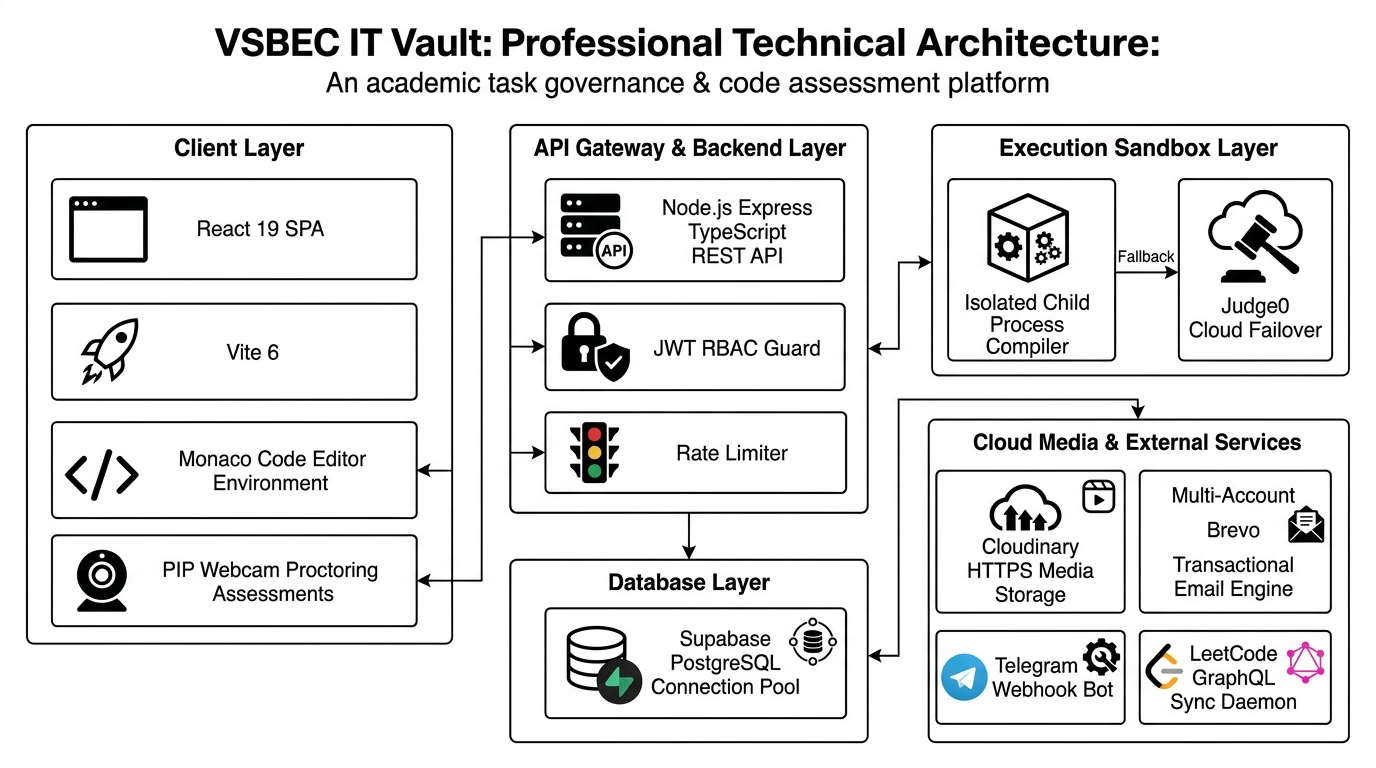
\includegraphics[width=0.92\textwidth,height=8.5cm,keepaspectratio]{images/system_architecture.png}%
  }\par
  \vspace{6pt}
  {\centering\fontsize{12pt}{16pt}\selectfont\bfseries Fig 5.1 System Architecture\par}
\end{figure}

\vspace{0.2cm}
{\fontsize{12pt}{17.5pt}\selectfont
As illustrated in Figure 5.1, the client presentation layer is built on React 19 and Vite 6, incorporating the Monaco code editor and Picture-in-Picture webcam proctoring. The API gateway enforces role-based route guards and rate limiting before dispatching requests to either the isolated compiler execution sandbox or the Judge0 cloud runtime. Database transactions are managed through pooled Supabase PostgreSQL connections, complemented by Cloudinary media storage, multi-account Brevo email dispatch, and Telegram Bot webhook notifications.\par}

\newpage

% --- PAGE 30: SECTION 5.2 MODULES USED ---
{\fontsize{14pt}{18pt}\selectfont\bfseries 5.2 MODULES USED\par}
\vspace{0.3cm}

Table 5.1 catalogs the primary production modules in the repository, their exact source code filepaths, and their architectural responsibilities.

\begin{table}[H]
  \centering
  \fontsize{10.5pt}{14.5pt}\selectfont
  \begin{tabularx}{\textwidth}{|p{4.2cm}|L|}
    \hline
    \textbf{Module Filepath} & \textbf{Architectural Scope and Implementation Responsibility} \\
    \hline
    \texttt{server.ts} & Express application root, REST API routing, RBAC route guard middleware, 3-tier task review endpoints, and proctoring telemetry traps. \\
    \hline
    \texttt{db.ts} & PostgreSQL database pooler, dynamic port 6543 rewrite for transaction pooling, custom INT8 and DATE type parsers, and DDL schema migration routines. \\
    \hline
    \texttt{codingSandboxService.ts} & Multi-language compiler jail (C, C++, Java 17, Python 3), 3000ms timeout traps, 64 KB buffer bounds, and Judge0 CE cloud failover runtime. \\
    \hline
    \texttt{emailService.ts} & Multi-account Brevo API load balancer (up to 5 account nodes), high-availability failover to Resend and SMTP, and 6-digit OTP email templates. \\
    \hline
    \texttt{telegramService.ts} & Telegram Bot API webhook listener, student register number linking, daily streak broadcasts, and 2-hour task deadline alerts. \\
    \hline
    \texttt{githubSyncService.ts} & Public GitHub REST event scraper, daily commit metrics extraction, and student portfolio data synchronization. \\
    \hline
    \texttt{.github/workflows/}\allowbreak\texttt{auto-backup.yml} & Automated disaster recovery workflow running at 07:50 AM and 11:55 PM IST, daily report compilation, and dual-remote GitHub sync. \\
    \hline
    \texttt{scripts/export-backup.ts} & LeetCode batch report generator, year/section CSV and JSON serializations, and full database JSON snapshot dumps. \\
    \hline
    \texttt{src/pages/}\allowbreak\texttt{StudentAssessment.tsx} & Monaco code editor interface, webcam Picture-in-Picture stream, HTML5 fullscreen lockdown, and tab-switch violation listeners. \\
    \hline
  \end{tabularx}
  \vspace{4pt}
  {\centering\fontsize{10.5pt}{14pt}\selectfont Table 5.1 System Modules and Source Code Implementation Mapping\par}
\end{table}

\vspace{0.3cm}
{\fontsize{14pt}{18pt}\selectfont\bfseries 5.3 MODULES DESCRIPTION AND DETAILED ENGINEERING LOGIC\par}
\vspace{0.2cm}
{\fontsize{13pt}{17pt}\selectfont\bfseries 5.3.1 Role-Based Access Control (RBAC) \& Route Guards\par}
\vspace{0.2cm}

{\fontsize{12pt}{17.5pt}\selectfont
This module governs authorization across six institutional roles: \texttt{SUPREME\_ADMIN}, \texttt{HOD}, \texttt{CLASS\_ADVISOR}, \texttt{STUDENT}, \texttt{COORDINATOR}, and \texttt{INDUSTRY}. Upon authentication, the server signs a cryptographically hardened JSON Web Token (JWT) using HMAC-SHA256:
\begin{equation}
T_{\text{jwt}} = \text{HMAC-SHA256}(\text{Base64}(H) \parallel \text{Base64}(P), K_{\text{jwt}}) \tag{1}
\end{equation}
where payload $P$ encapsulates the user ID, role, department ID, and class scope. Every API endpoint enforces role middleware that validates bearer tokens and rejects unauthorized requests with HTTP 403 Forbidden. Passwords are cryptographically salted and hashed using \texttt{bcryptjs} with 10 salt rounds before storage.

\vspace{0.4cm}
{\fontsize{13pt}{17pt}\selectfont\bfseries 5.3.2 3-Tier Hierarchical Verification Pipeline \& Cloud Asset Lifecycle\par}
\vspace{0.2cm}

The core academic workflow enforces an auditable multi-tier verification finite state machine (FSM). When a student submits task evidence (source code, screenshots, and custom fields), the submission transitions across deterministic lifecycle states:
\begin{align}
S_0 (\text{PENDING}) &\xrightarrow{\text{submit}} S_1 (\text{SUBMITTED}) \xrightarrow{\text{audit}_{\text{coord}}} S_2 (\text{PEER\_VERIFIED}) \notag \\
&\xrightarrow{\text{review}_{\text{advisor}}} S_3 (\text{VERIFIED}) \tag{2}
\end{align}

If deficiencies are detected at any tier, the reviewer triggers a state rollback:
\begin{equation}
S_{\text{current}} \xrightarrow{\text{reject}(\text{reason})} S_{\text{rejected}}, \quad \text{resubmission\_count} \leftarrow \text{resubmission\_count} + 1 \tag{3}
\end{equation}

All uploaded evidence assets are streamed directly to Cloudinary using signed multipart uploads via \texttt{multer-storage-cloudinary}. The PostgreSQL database stores the secure HTTPS delivery URL alongside the Cloudinary \texttt{public\_id}. When a student resubmits or when an assignment concludes, an automated storage cleanup daemon purges stale screenshots from Cloudinary storage to maintain zero unnecessary cloud storage overhead. Every status transition creates an immutable record in \texttt{submission\_reviews} capturing the reviewer UUID, previous status, new status, and feedback text.

\vspace{0.4cm}
{\fontsize{13pt}{17pt}\selectfont\bfseries 5.3.3 Multi-Language Sandboxed Compiler Engine \& Judge0 Failover\par}
\vspace{0.2cm}

The coding assessment subsystem executes untrusted student source code in C, C++, Java 17, and Python 3. To defend against resource exhaustion, denial of service, and directory traversal, execution is isolated within sandboxed child processes spawned with a sanitized environment:
\begin{equation}
\mathcal{E}_{\text{clean}} = \{\text{PATH}, \text{TEMP}, \text{TMP}, \text{COMSPEC}, \text{SYSTEMROOT}\} \tag{4}
\end{equation}

A strict timeout trap enforces execution boundaries:
\begin{equation}
\Delta t \le T_{\text{limit}} \quad (T_{\text{limit}} = 3000\text{ ms}) \tag{5}
\end{equation}
If execution exceeds $T_{\text{limit}}$, a \texttt{SIGKILL} signal terminates the child process tree immediately, returning status \texttt{TIME\_LIMIT\_EXCEEDED}. Output streams (\texttt{stdout} and \texttt{stderr}) are capped at 64 KB to eliminate buffer overflow attacks.

In serverless production environments (such as Vercel Edge functions where local compilers like \texttt{gcc} or \texttt{javac} are unavailable), the engine automatically activates a resilient cloud failover to the Judge0 CE API. The engine wraps Java source code into \texttt{public class Main}, formats stdin streams, and executes test batches concurrently with exponential backoff retry logic.

\vspace{0.4cm}
{\fontsize{13pt}{17pt}\selectfont\bfseries 5.3.4 LeetCode GraphQL \& GitHub Commit Telemetry Daemons\par}
\vspace{0.2cm}

To continuously monitor algorithmic momentum, background daemons execute scheduled polling routines every 24 hours. The LeetCode daemon issues a GraphQL query against the LeetCode public API endpoint:
\begin{equation}
Q_{\text{leetcode}} = \text{GraphQL}(\text{username}, \text{matchedUser}\{\text{submitStatsGlobal}\{\dots\}\}) \tag{6}
\end{equation}

The response payload is parsed to compute total solved problems, difficulty distribution (Easy, Medium, Hard), and daily delta solve velocity:
\begin{equation}
\Delta N_{\text{today}} = N_{\text{total}}(t) - N_{\text{total}}(t - 1) \tag{7}
\end{equation}
Records are persisted idempotently into the \texttt{leetcode\_daily\_progress} table. Simultaneously, the GitHub sync engine interfaces with the GitHub REST API endpoint for public user events, filtering for \texttt{PushEvent} payloads occurring on date $D$. The total daily commits are computed:
\begin{equation}
C_{\text{daily}} = \sum_{e \in \text{PushEvents}} \text{len}(e.\text{commits}) \tag{8}
\end{equation}
and upserted into \texttt{github\_daily\_commits}. Class-level and department-level leaderboards are computed dynamically from these indexed relational tables.

\vspace{0.4cm}
{\fontsize{13pt}{17pt}\selectfont\bfseries 5.3.5 Automated Disaster Recovery and Dual-Repository Backup Workflow\par}
\vspace{0.2cm}

A unique differentiating capability of this codebase is its fully automated disaster recovery pipeline orchestrated via GitHub Actions in \texttt{.github/workflows/auto-backup.yml}. The workflow runs autonomously on two daily cron schedules:
\begin{itemize}[noitemsep,topsep=2pt,leftmargin=*]
  \item \textbf{07:50 AM IST (\texttt{20 2 * * * UTC}):} Morning pre-sync and previous day cumulative report snapshot.
  \item \textbf{11:55 PM IST (\texttt{25 18 * * * UTC}):} Nightly final daily report and complete database JSON snapshot backup.
\end{itemize}

The workflow executes \texttt{npx tsx scripts/export-backup.ts}, which queries PostgreSQL via connection pooling and generates master CSV reports (\texttt{leetcode/LeetCode\_Daily\_Report\_YYYY-MM-DD.csv}), year-wise/section-wise CSV and JSON files, and full database relational snapshots saved to \texttt{backups/db\_backup\_*.json}. The workflow then automatically commits these artifacts with the message \texttt{chore(backup): auto-snapshot database and reports...} and pushes to the primary GitHub remote. Crucially, if a synchronization token (\texttt{SYNC\_PAT}) is configured, the workflow automatically synchronizes the commit to the mirror repository, guaranteeing 100\% parity between \texttt{TK4743/taskmanager} and \texttt{Tharun4743/taskmanager} with zero human intervention.

\vspace{0.4cm}
{\fontsize{13pt}{17pt}\selectfont\bfseries 5.3.6 High-Availability Multi-Account Brevo Transactional Email Engine\par}
\vspace{0.2cm}

Authentication security and password recovery depend on a dedicated multi-account Brevo transactional email engine implemented in \texttt{emailService.ts}. Rather than relying on a single API key that can be blocked or exhausted, the system establishes a load-balancing pool supporting up to 5 Brevo account nodes:
\begin{equation}
\mathcal{N}_{\text{brevo}} = \{\text{Node}_1, \text{Node}_2, \text{Node}_3, \text{Node}_4, \text{Node}_5\}
\end{equation}

When dispatching emails, the pool checks node quota health via \texttt{GET https://api.brevo.com/v3/account} and load balances requests across active nodes with 50ms pacing. If all Brevo nodes are exhausted or encounter network timeouts, the system automatically falls back to the Resend API or direct authenticated SMTP relays.

For password resets, the server generates a cryptographically random 6-digit numerical OTP, creates an audit record in the \texttt{password\_resets} table with an exact 10-minute expiration window (\texttt{expires\_at}), and enforces a strict rate limit of at most 5 attempts before invalidating the code.

\vspace{0.4cm}
{\fontsize{13pt}{17pt}\selectfont\bfseries 5.3.7 Tri-Channel Notification Dispatcher\par}
\vspace{0.2cm}

To eliminate deadline miss rates, the platform deploys a tri-channel notification engine integrating Telegram Webhooks, Web Push (VAPID), and transactional email.
Students link their Telegram accounts by sending their university register number to the department bot. Automated routines dispatch morning LeetCode streaks, 2-hour task deadline alerts, and verification status updates via the Telegram Bot API:
\begin{equation}
R_{\text{telegram}} = \text{POST}(\text{API}_{\text{telegram}} \parallel \text{token}, \{\text{chat\_id}, \text{text}, \text{parse\_mode}\}) \tag{9}
\end{equation}
Concurrently, lockscreen push notifications are dispatched to browsers via VAPID service workers over elliptic curve P-256 keys.

\vspace{0.4cm}
{\fontsize{13pt}{17pt}\selectfont\bfseries 5.3.8 Picture-in-Picture (PIP) Anti-Cheat Proctoring Engine\par}
\vspace{0.2cm}

During corporate placement tests and department coding assessments, the platform enforces client-side browser proctoring without requiring invasive operating system agents.
The client initiates a video stream via \texttt{navigator.mediaDevices.getUserMedia()} rendered inside a Picture-in-Picture floating viewport. Periodic canvas snapshot frames are uploaded to Cloudinary as visual proctoring audit trails.
Assessments mandate fullscreen mode via the HTML5 Fullscreen API:
\begin{equation}
\text{requestFullscreen}() \quad \text{with listener on } \texttt{fullscreenchange} \tag{10}
\end{equation}
Any attempt to minimize or exit fullscreen triggers an immediate modal lockout overlay. The platform attaches event listeners to \texttt{document.visibilityState} and \texttt{window.onblur}. When a student shifts focus away from the test tab, a violation event is recorded:
\begin{equation}
E_{\text{violation}} = \{\text{type}: \text{``TAB\_SWITCH''}, \text{timestamp}: t, \text{duration}: \Delta t_{\text{blur}}\} \tag{11}
\end{equation}
Violations are accumulated in the \texttt{student\_assessments.integrity\_events} JSONB column. If violations exceed the threshold, the assessment auto-submits.

\vspace{0.4cm}
{\fontsize{13pt}{17pt}\selectfont\bfseries 5.3.9 Corporate Industry Portal \& Placement Readiness Index\par}
\vspace{0.2cm}

The corporate module bridges academic achievements with corporate recruitment drives. Industry partners post opportunities with custom eligibility criteria. When an assessment launches, the question bank is dynamically shuffled so that each student receives a randomized question subset.
The system computes an empirical Placement Readiness Index score ($P_{\text{index}} \in [0, 100]$):
\begin{multline}
P_{\text{index}} = w_1 \cdot \left(\frac{\text{CGPA}}{10} \times 100\right) + w_2 \cdot \min\left(100, \frac{N_{\text{Leet}}}{300} \times 100\right) \\
+ w_3 \cdot S_{\text{assess}} + w_4 \cdot \min\left(100, \frac{C_{\text{Git}}}{150} \times 100\right) \tag{12}
\end{multline}
where $w_1 = 0.30$, $w_2 = 0.30$, $w_3 = 0.25$, and $w_4 = 0.15$. Placement coordinators can generate filtered student dossiers exported in Microsoft Excel (.xlsx) and Adobe PDF formats with a single click.\par}
\newpage
